\section{Implementation} \label{implementation}

\subsection{Lexing \& Parsing}
\label{syntax}
Looking at the lexical syntax within section 10.1 of the Haskell 2010 Language Report\cite{haskell2010} there are many reused notational constructs, shown in Table \ref{tab:lexical-notation}. Due to this, I identified using a lexer combinator as the ideal choice for lexing.

A lexer combinator is a higher-order function that accepts one or more lexer, and returns a new lexer. When this lexer is run against an input, it returns an array containing all the possible matches. This quickly allows for complex lexers to be implemented, and for additional rules to be added.
I first set about creating the lexers that represent the notational constructs given, as well as the maximal munch rule, shown in \ref{tab:lexical-constructs}.
\begin{figure}
    \centering
    \begin{lstlisting}[language=JavaScript]
function any(...fs) {
    // Attempt to lex against each choice, returning all matches.
    return (input) => fs.map(f => lexer(f)(input));
}\end{lstlisting}
    \caption{The lexer corresponding to the choice rule, returning all matches.}
    \label{fig:any-lexer}
\end{figure}
This rule requires the longest input to be consumed at each step. This is especially apparent when matching identifiers, as it solves the problem of the identifier ``letter'' being lexed as the keyword ``let'' and the identifier ``ter''.
With these building blocks, all the other lexers could be quickly constructed, such as the lexer responsible for marking variable identifiers (used for type variables, function identifiers, and arguments).
\begin{figure}
    \centering
    \begin{lstlisting}[language=JavaScript]
varid = tok(diff(all(small, many(any(small, large, digit, "'"))), reservedid), Token.VARID)\end{lstlisting}
    \caption{
    {\it varid} $\rightarrow$ ({\it small}\{{\it small}$|${\it large}$|${\it digit}$|${\tt '}\})$_{\langle revservedid\rangle}$
    }
    \label{fig:varid-lexer}
\end{figure}
A benefit of using a lexer combinator, was that each parser could be individually tested before constructing the next one. For example, the ``varid'' parser depends on a number of smaller parsers. Once I knew the smaller parsers were working correctly, I could confidently rule them out as the causes for issues. This allowed for rapid prototyping, and lexing hence took a short time to implement.

Once the input had been lexed, it could then be converted into the internal representation, described in section \ref{internals}. This would also use an LL parser but, due to the complexity of converting from tokens to thunks, was not implemented as a parser combinator. A top down parser was still used for simplicity.

The further goals of this project, data types and type classes, both rely on specific keywords (data, and class and instance respectively). In fact no keywords were initially required, as other keyword expressions (case-of, if-then-else, foreign, e.t.c) were not planned to be supported. This allowed the basics to be implemented, before more complicated structures were parsed.

As the tokens were in an ordered list, they could be shifted off of a queue, inspected, and then a decision made. If an invalid token was received, an error was thrown, which describes what token it encountered, what token it expected, and where in the user input it happened. This allows the user to modify their code quickly, and handle the errors they encounter one at a time.

Parsing of each construct was implemented inside a dedicated function. Some functions iterate other the tokens until a specific end token is found, such as a $\Rightarrow$, or a close parenthesis, and others simply parse until the end of the line (new lines are the only whitespace preserved by the lexer). By using separate functions, each construct could be parsed and tested individually, and can use each other when required.

As they are parsed, functions, data types, and type classes are stored under the "main" module. As the input is parsed from the top down, constructs must be defined before they are used. For example, when an identifier is seen within a function, if it exists as an already parsed function, it is recorded as a call to that function. Otherwise, it is recorded as an unbound identifier.

The full grammar of the language is described in Figure \ref{fig:grammar}.

\subsection{Internals} \label{internals}
Before implementing the parser, I had to create the internal representation that the user input would parse into.

\subsubsection{Types}
\begin{figure}
\centering

\begin{tikzpicture}[scale=2,
type/.style = {
    rectangle, rounded corners,
    draw=black, fill=blue!40, drop shadow,
    text centered, anchor=north, text=white, text width=2.6cm,
},
arrow/.style = {
    shorten >= 0.33cm, shorten <= 0.33cm
}]

\node (root)  [type, text width=6cm] at (0, 2) {FunctionType\\(a $\rightarrow$ Integer) $\rightarrow$ a $\rightarrow$ Integer};
\node (lFunc) [type] at (-1.8, 1) {FunctionType\\a $\rightarrow$ Integer};
\node (rFunc) [type] at (1.8, 1) {FunctionType\\a $\rightarrow$ Integer};
\node (lA)    [type] at (-2.7, 0) {UnboundType\\a};
\node (rA)    [type] at (0.9, 0) {UnboundType\\a};
\node (lInt)  [type] at (-0.9, 0) {LiteralType\\Integer};
\node (rInt)  [type] at (2.7, 0) {LiteralType\\Integer};

\draw[->, arrow] (root) -- (lFunc);
\draw[->, arrow] (root) -- (rFunc);
\draw[->, arrow] (lFunc) -- (lA);
\draw[->, arrow] (lFunc) -- (lInt);
\draw[->, arrow] (rFunc) -- (rA);
\draw[->, arrow] (rFunc) -- (rInt);

\end{tikzpicture}

\caption{The internal representation of: (a $\rightarrow$ Integer) $\rightarrow$ a $\rightarrow$ Integer}
\label{fig:a-int--a-int}
    
\end{figure}
Haskell does not have a dependant type system, which means that while thunks would depend on types, types would not depend on thunks. This meant I could implement and test them first before moving on to thunks. As planned, types were constructed as a tree, allowing types to be built using other types, as in Figure \ref{fig:a-int--a-int}. Initially, only literal, unbound, and function types were implemented, with no notion of typeclasses, to create the first prototype. These were enough to create basic functions.

However, before they could work, a method of type inference was required. For example, if a {\tt String $\rightarrow$ Integer} function is bound to the type in Figure \ref{fig:a-int--a-int}, it is inferred that {\tt a} is the type {\tt String}, and the type {\tt String $\rightarrow$ Integer} would be returned. This is performed by first collecting all of the type constraints, before unifying them using a variation of the algorithm presented in \cite{unification}. This reduces the constraints until either a solved set is created, or an error is thrown, indicating a badly typed expression.

The simplest matching was for LiteralTypes, which had to be identical (so an \texttt{Integer} could match an \texttt{Integer}, but not a \texttt{Bool}), and generated no constraints.
FunctionTypes simply had to match their left and right children to the left and right child of the incoming type (which also had to be a FunctionType). It returned the union of the constraints of its children.
UnboundTypes were by far the most complicated. Given two types with disjoint sets of unbound symbols, they could simply match together, with the constraint setting them equal. However, if the symbol sets were not disjoint, matching has additional constraints. This is solved by introducing a strict set, where matching can only occur against identical symbols within the set, but any symbol outside of the set. In Figure \ref{fig:disjoint}, ``f'' has the strict set ``\{a, b\}'', so when an ``a'' tries to match a ``b'', it fails. When the second argument's type is changed to an ``a'', it is able to successfully match an ``a'' to an ``a'' and succeeds. 
\begin{figure}
    \centering
    \begin{lstlisting}[language=Haskell]
foo :: (a -> b) -> b -> b
foo f b = f b\end{lstlisting}
    \caption{``foo'' actually has the type ``$\forall a. \forall b. (a\rightarrow b)\rightarrow b\rightarrow b$'', which fails as `b' can only be bound to ``a $\rightarrow$ b'' when ``a'' and ``b'' are equal, not for all ``a'' and ``b''.}
    \label{fig:disjoint}
\end{figure}
UnboundTypes also have one other opportunity to match. Whenever the incoming type is an UnboundType, matching is also performed in the other direction. This is required as constraining a variable within the incoming type may constrain other variables in both the incoming and receiving type.

Data types were relatively simple to add. Just like LiteralTypes (such as \texttt{Integer} and \texttt{Bool}\footnote{\texttt{Bool} is actually implemented as a data type, but as it has no variables behaves identically to a LiteralType.}, the names of the type must match exactly. You can't substitute a \texttt{Maybe} for an \texttt{Either}, just like you can't substitute a \texttt{String} for an \texttt{Integer}. The similarities meant that instead of creating a new class for these, LiteralType worked perfectly with no changes.
Types which had arguments relied on a new class, ApplicationType, which had a left and right child. They matched identically to FunctionTypes, as their left and right children had to match, and the generated constraints were unioned.

The last feature to implement for types were type classes. Additional constraints to unbound types about what types could replace them. Due to the modular implementation, this only required additional logic to be added to the UnboundType class for checking if a binding was valid. Incoming types had to be at least as restrictive as the receiving type, e.g ``Real c => c'' is more restrictive than ``Num a => a'', as the ``Real'' type class depends on the ``Num'' type class, whereas ``b'' (with no constraints) is less restrictive and cannot match. When a LiteralType is bound to an UnboundType, it now required the LiteralType to have implemented whichever constraints the UnboundType held.  

\subsubsection{Thunks}
Like types, thunks were implemented incrementally with a specific interface. To begin with, only 4 thunks were needed: literal, unbound, function, and application. These directly correspond to the types of the same name, with the ApplicationThunk corresponding to applying a type to a function type. Also like types, each child thunk of a thunk was to be a valid thunk by itself, allowing them to be passed around and substitued where required.

A LiteralThunk represents an actual value, such as the number 1, the float 1.0, or the character 'a', and, as its type is known at compile time, is annotated with its type. By annotating as many thunks as possible as early as possible, type inference and type checking takes less time, and provides stricter results.
An UnboundThunk represents an unknown value, typically found in the arguments. It only needs to know which symbol it is represented by. It is initialised with an AllType, as it could have any value on its own.
An ApplicationThunk represents an application of one thunk to another. It takes its two child thunks as arguments. When this thunk is asked for its type, it uses a JavaScript getter method to dynamically infer its type from its children. This also ensures that its left child is always a type of function. The ApplicationThunk is the first thunk that can "step", evaluating one step of computation. If the left child is an ApplicationThunk, or otherwise can step, then it must step before the right child can be applied. However the right child does not always need to be stepped to be applied, because of the call-by-need evaluation strategy.

A FunctionThunk represents an individual function. When creating a function, initially it just needs a name and a type. This allows it to be initialised, and then used in function definitions for recursion. A function with no cases is equivalent to $\bot$, and will throw an error if it is attempted to be called. Cases are added by defining a pattern and an implementation. The implementation is simply a thunk, but the pattern is a specific class, essentially a wrapper around a list of arguments.

When an ApplicationThunk applies a thunk to a function, it first evaluates the resultant type. During evaluation this is guaranteed to succeed, as the types of functions and expressions are checked after parsing. Then each pattern is checked for a match, which is described in Section \ref{args}. 
If the match fails, then the pattern and relevant implementation are discarded, as there's no way for the function to evaluate that branch. If the match succeeds the pattern discards the matched argument, and either sets a new case for the resultant FunctionThunk, or (if the pattern matched completely) returns the relevant implementation.
If, after matching, no patterns are left in the resultant FunctionThunk, then it means all matches failed (and the pattern matching was incomplete), which is equivalent to $\bot$ and a helpful error is thrown, shown in Figure \ref{fig:incomplete}.
Like in Haskell, a partially matched function is a function of its own, and can be parsed around like any other thunk.

\begin{figure}
    \centering
    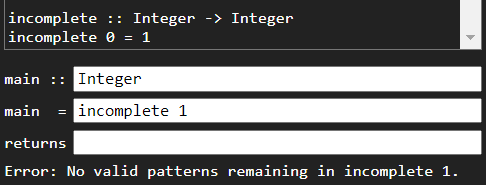
\includegraphics[scale=0.75]{chapters/5-implementation/images/incomplete.png}
    \caption{Incomplete functions will error if no cases match.}
    \label{fig:incomplete}
\end{figure}

Not all computation is easy to define using Haskell alone. Int addition could be defined with lines upon lines of pattern matching, but this is impractical in the best cases, and impossible (e.g for types with infinite constructors such as Integer) in the worst cases. In these cases Haskell defers to C but, to keep it available to use on the web, we will defer to JavaScript. These functions, called JSThunks, are restricted to using a subset of types. JavaScript has no notion of the type "Either a b", IO types, and many more, but it does contain numbers, characters, strings, and arrays, which have corresponding types in Haskell.
To implement these, they require a name, a type, and a JavaScript function. Again, as Haskell allows all functions to be curried, and can be partially applied. This is solved for JSThunks by passing in a function that returns a function.
\begin{lstlisting}[language=JavaScript, caption=A curried addition function in JavaScript.]
((a, b) => a+b)(1, 2)
(a => b => a+b)(1)(2)
\end{lstlisting}
Whenever a JSThunk's function returned a new function, it was wrapped in a new JSThunk with the appropriate name and type. If the value being returned was to be a Literal, it was wrapped in a LiteralThunk, and given the type inferred from the function and argument's types, allowing basic polymorphism. Lastly, (once data types had been implemented), specific data types were supported, such as converting JavaScript's primitive true and false, to Haskell's True and False constructors, as well as converting strings to and from character lists to JavaScript strings.
To simplify JSThunks, they do not perform any pattern matching. This could be emulated using if-else statements in their JavaScript functions, as could any arbitrary function. This was specifically avoided to keep computation within the interpreted Haskell environment as much as possible, to ensure as much could be visualised as possible. This is because JavaScript execution, such as adding or multiplying 2 numbers isn't visualised step by step. If, for example, the n$^{th}$ Fibonacci number was implemented as a JSThunk, instead of a regular FunctionThunk, the user would not be able to see each step be visualised. It would jump from the function call to the final answer, instead of showing the recursive calculation.

With data types, ConstructorThunks were introduced. These behave similarly to LiteralThunks, but their type is defined within the data type declaration. Essentially they are a LiteralThunk which has a FunctionType.

With type classes, their methods can behave completely differently depending on which instance method is required. Which method is required is determined by the type of its arguments and return value. To fix this, FunctionReferenceThunk was introduced.
When a class method is parsed, the number of arguments that must be applied to it to determine which instance to use. When the FunctionReferenceThunk has enough arguments applied, it reduces to the specific form of the method. For example, the fmap function in Figure \ref{fig:fmap}, which is dependant on the ``m'' type variable to decide which ``Moand'' instance is used. When the List Monad is used it behaves like the standard ``map'' function, but when the Maybe Monad is used it propagates ``Nothing'', and only applies the function within the ``Just'' case.
\begin{figure}
    \centering
    \begin{lstlisting}[language=Haskell]
fmap :: (a -> b) -> m a -> m b
fmap f ? = ?\end{lstlisting}
    \caption{fmap}
    \label{fig:fmap}
\end{figure}

\subsubsection{Arguments}
\label{args}
As described above, FunctionThunks use Patterns, which wrap a list of Arguments. The initial arguments, either literals or unbound, would match either literals, or anything respectively.
When matching a LiteralThunk to a LiteralArgument, their types and values must be the same, or else they fail. If the thunk passed to a LiteralArgument is not fully evaluated, it must be. This is because an unevaluated thunk, despite having a fixed type inferred from its children, does not have a fixed value. As in Figure \ref{fig:requires-steps}, no assumption can be made about what ``$(1+1)$'' might return, other than it will return an ``Integer''.
When matching an UnboundArgument, only the type was required to match, and the symbol used for the argument is replaced within the corresponding implementation. This type of argument doesn't require a thunk to be evaluated, allowing for the call-by-need evaluation strategy. In the second case of Figure \ref{fig:requires-steps}, as ``a'' is not required to be a specific value, ``$(1+1)$'' does not need to be evaluated.
A special argument, the WildcardArgument, written in Haskell as an underscore is the same as an UnboundArgument, except no replacements occur when a match succeeds. There can also be multiple wildcards within a single pattern, unlike the symbols of unbound arguments.
\begin{figure}[h]
    \centering
    \begin{lstlisting}[language=Haskell]
foo :: Integer -> Integer
foo 0 = 1
foo a = a
foo _ = 0

main = foo (1+1)\end{lstlisting}
    \caption{$(1+1)$ must be evaluated before the pattern can test each match.}
    \label{fig:requires-steps}
\end{figure}

To go through step by step, in Figure \ref{fig:requires-steps}, ``$(1+1)$'' is compared to ``0''. As the argument is an unevaluated thunk, instead of continuing to match against the other cases, the argument is evaluated, leaving the expression as ``foo 2''. If matching was allowed to continue, a unevaluated thunk that represented the value ``0'' could erroneously match later cases. In the next step, ``2'' is first compared to ``0''. While their types match, their values do not, so the ``foo 0 = 1'' case is discarded. Then ``2'' is compared to ``a''. As ``a'' is unbound, it accepts all arguments, and the match returns the constraint ``a = 2''. This constraint is applied to the implementation, setting the UnboundThunk ``a'', to the LiteralThunk ``2''. As ``a'' was the final argument in ``foo'', the case has been fully matched, and so the second case is returned.
While ``$(1+1)$'' could also match on the third case, as it is a wildcard, only the first successful match is returned. This allows some cases to be more restrictive (such as the ``0'' case as shown) and take precedence over less restrictive cases.

Introducing data types to arguments came with some challenges.
While the matching of ConstructorArguments and ApplicationArguments was simple, with ConstructorArguments having to match exactly, and ApplicationArguments having to match their children. Annotating the types of arguments was initially challenging.
As a data type's constructors can be of many different forms inside the same data type. The type that the constructor returns must first be fetched, and then matched against the expected type of the argument, and potentially restricting some types. In Figure \ref{fig:datatype}, while the first case's symbol match the order of ``Foo'', the second cases does not. Assuming the constructor returns type checks so returns the correct type, the type and order of arguments must be deduced through the constructor.
\begin{figure}
    \centering
    \begin{lstlisting}[language=Haskell]
data Foo a b c = Unit
               | Fixed Integer
               | Var a b c
               | Reverse c b a
               | Omit a c

example :: Foo Integer String Bool -> Foo a b c
example (Var u v w)     = Unit
example (Reverse x y z) = Fixed 1
\end{lstlisting}
    \caption{While all of ``Foo'''s constructors return a value of ``Foo a b c'', the order of their arguments (if any) can differ from the order in the declaration.}
    \label{fig:datatype}
\end{figure}

When implemented, typeclasses slotted in seamlessly, as they were implemented completely separately of arguments and thunks. When matching types, because the methods defined in the Type interface were used, once changes to those methods were successfully implemented, users of those methods were able to work with typeclasses with no additional changes.

\subsection{Visualising}
\subsubsection{UI \& User Input}
\begin{figure}
    \centering
    \begin{minipage}[b]{0.45\textwidth}
        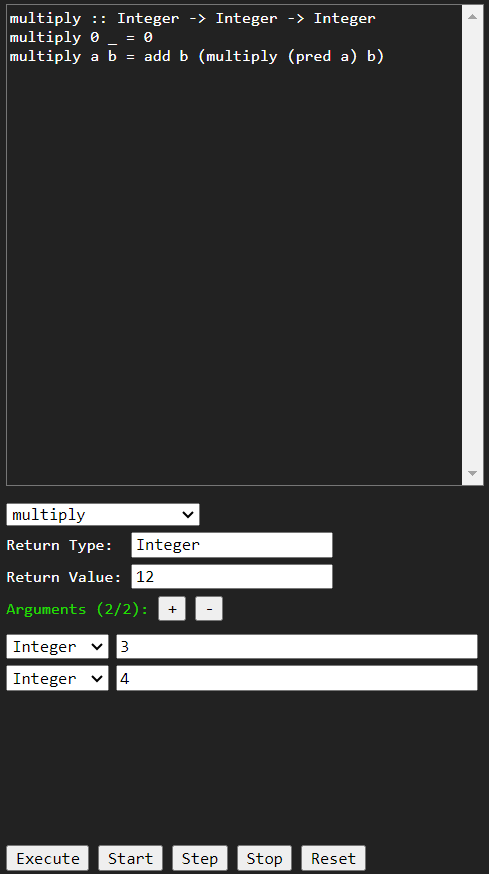
\includegraphics[width=\textwidth]{chapters/5-implementation/images/old.png}
        \caption{The first iteration of the UI.}
        \label{fig:old-ui}
    \end{minipage}
    \hfill
    \begin{minipage}[b]{0.45\textwidth}
        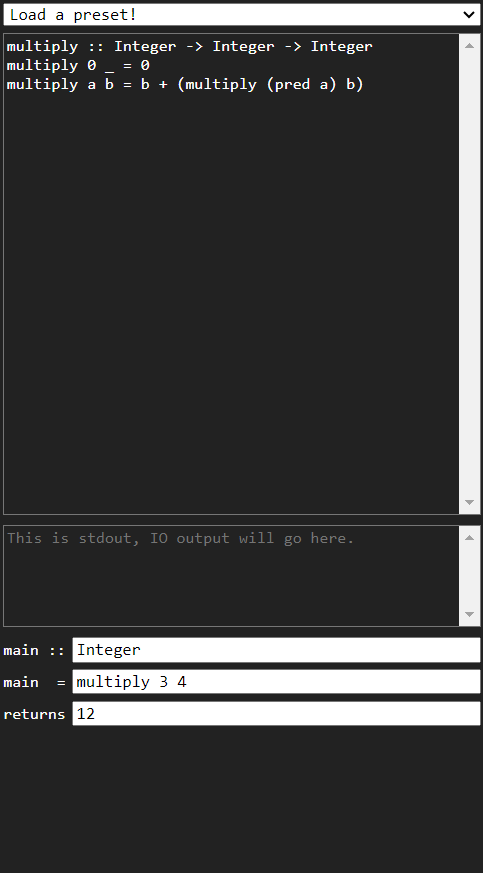
\includegraphics[width=\textwidth]{chapters/5-implementation/images/new.png}
        \caption{The second iteration of the UI.}
        \label{fig:new-ui}
    \end{minipage}
\end{figure}
\begin{figure}
    \centering
    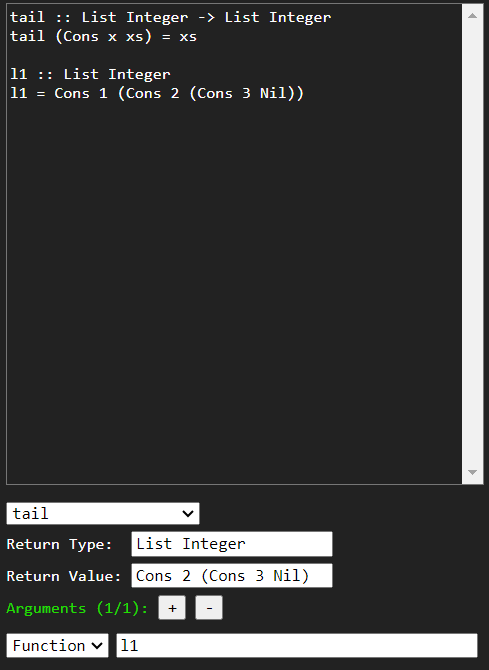
\includegraphics[width=0.9\linewidth]{chapters/5-implementation/images/awkward.png}
    \caption{An inelegant fix to bad UI.}
    \label{fig:awkward}
\end{figure}
The UI, and how the user input a program underwent through two major iterations during development.

Initially, as shown in Figure \ref{fig:old-ui}, the user would input a program within the topmost box. Using the input boxes below, the user could then select a function to evaluate and determine the number of arguments to pass into it (using the + and - buttons). The text would turn green when enough arguments are being passed into the chosen function. To choose arguments, the type could be selected from a drop down list, either ``Integer'', ``Float'', ``String'', or ``Function''. ``Function'' allowed the user to set the argument as a function they had defined in the code input box. The values, such as a number, a string, or the name of a function, could be input in the box to the right of the type.
The buttons at the bottom controlled the evaluation of the expression. ``Evaluate'' would fully evaluate the expression, putting the return type and value into the relevant boxes once finished.
``Start'' and ``Stop'' would enable and disable stepping through the expression five times a second.
``Step'' would step once through the evaluation and, if the expression had finished evaluating, fill the return type and value boxes.
``Reset'' would reset the expression back to the beginning, so the user could step through it again.

While functional, this iteration had numerous drawbacks. The main two were how slow it was to setup evaluation, and how data types could not be easily integrated. Any function could be run, but defining the arguments one by one, and manually setting their type was both tedious and error prone. The user could input a string, but set its type as an ``Integer'' which could cause unintended issues\footnote{Though because of JavaScript's automatic type conversion usually didn't cause any JavaScript errors.}.
As this version of the UI was made before data types had been implemented, when they were added an elegant solution for the user to user data types in their arguments was not possible. The easiest way was for the user to define a new function, which took no arguments, and returned the specific data type they wanted, such as in Figure \ref{fig:awkward}.

The second iteration of the UI, shown in \ref{fig:new-ui}, was the result of fixing the problems of the first iteration, new features, and especially user feedback. The main change was switching from setting individual arguments, to a ``main'' function. This was implemented by simply parsing the expression within the main function input box. This could automatically work out the types of the arguments, as well as parse more complicated expressions such as those used to make data types. This box was strictly limited to parsing function implementations (as it was the implementation of ``main'', and can even be used recursively), so when the parser was expanded, the capabilities of ``main'' also expanded. Haskell usually restricts this function to the ``IO ()'' type, but, as it was the only entry point, it was relaxed to allow any return type.
This UI also has the additional feature of live evaluation. Whenever the expression does not depend on user input, the expression will be evaluated to attempt to find the return type and value. If these are found within a couple seconds, they are displayed to the user. These values help the user quickly debug programs, as if the return type or value doesn't match what they thought it would, they can edit their program, and see the new changes live. 

When monadic IO was implemented, a new read-only box was added for IO output to display. IO input was naturally implemented through JavaScript's modals, as they can easily request a line of input from the user when run.

\subsubsection{Expressions}
Visualising expressions was the core method for the user to learn and understand functional concepts. Figure \ref{fig:broad-example} shows an expression mid evaluation, as well as showing some type information and sub-expressions.

Instead of multiple control buttons, as in the first iteration of the UI in Figure \ref{fig:old-ui}, the right hand side can instead be clicked on to evaluate a single step. The user can click on the ``T'' button to open up the type information box, and close it with the ``X'' button. This box shows the type information of the corresponding expression. This is useful as every sub-expression is also a valid expression with it's own type, so the user can use this information to see why types are the way they are. For example, in Figure \ref{fig:broad-example}, the type of the full expression is ``Either Integer Bool'', which is made by combining the type of the two sub-expressions within the ``ite'' function, which have the ``Either Integer a'' and ``Either a Bool'' type respectively.

\begin{figure}
    \centering
    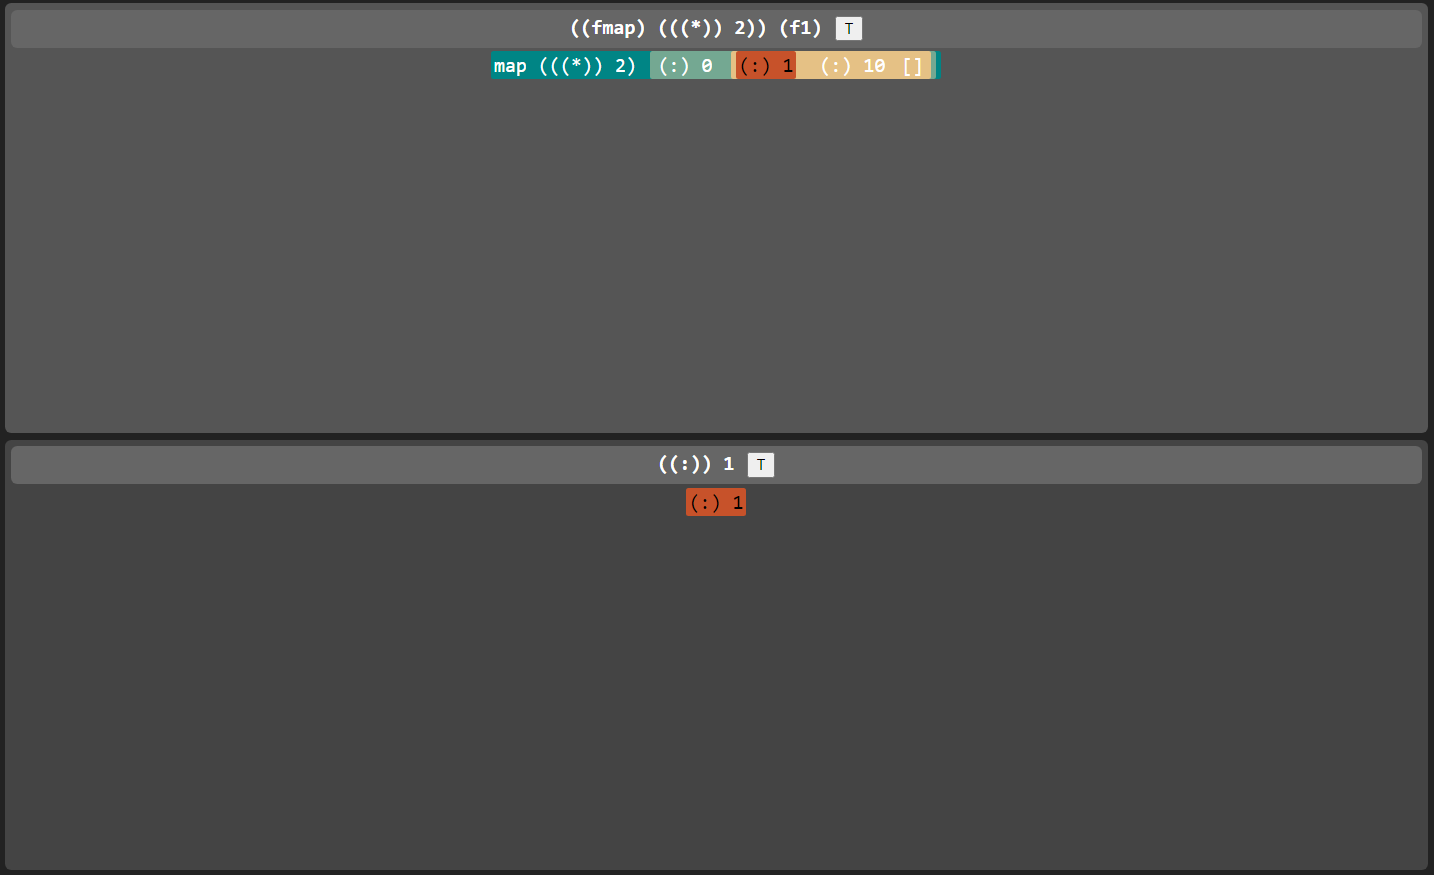
\includegraphics[width=\linewidth]{chapters/5-implementation/images/hover.png}
    \caption{When hovering over an application, it, and its parents, are highlighted, including within sub-expressions.}
    \label{fig:hover}
\end{figure}
To open up a sub-expression, the user can click on part of an expression. In Figure \ref{fig:hover}, the ``((:) 1)'' expression has been clicked, opening it up below. In this case, it can't be evaluated further, but if it can, when the below box is clicked, it is evaluated separately from the main expression. This allows the user to experiment with parts of expressions, without them affecting the main expression. Once fully evaluated, it can be clicked again to be removed. Thunks which are the same object, such as ``(:) 1'' in both the main and sub-expressions, are highlighted the same colour when hovered, to show that they are linked. 3 layers of applications above of the hovered-over thunk are also highlighted, to show where it exists in relation to the rest of the expression.